\section{Structuring Machine Learning Projects}
This is the third course of deep learning specialization at Coursera taught by Professor Andrew Ng. Here is my certificate after finishing this course (Fig. \ref{C3-Certificate}):

\begin{figure}[!htbp]
    \centering
    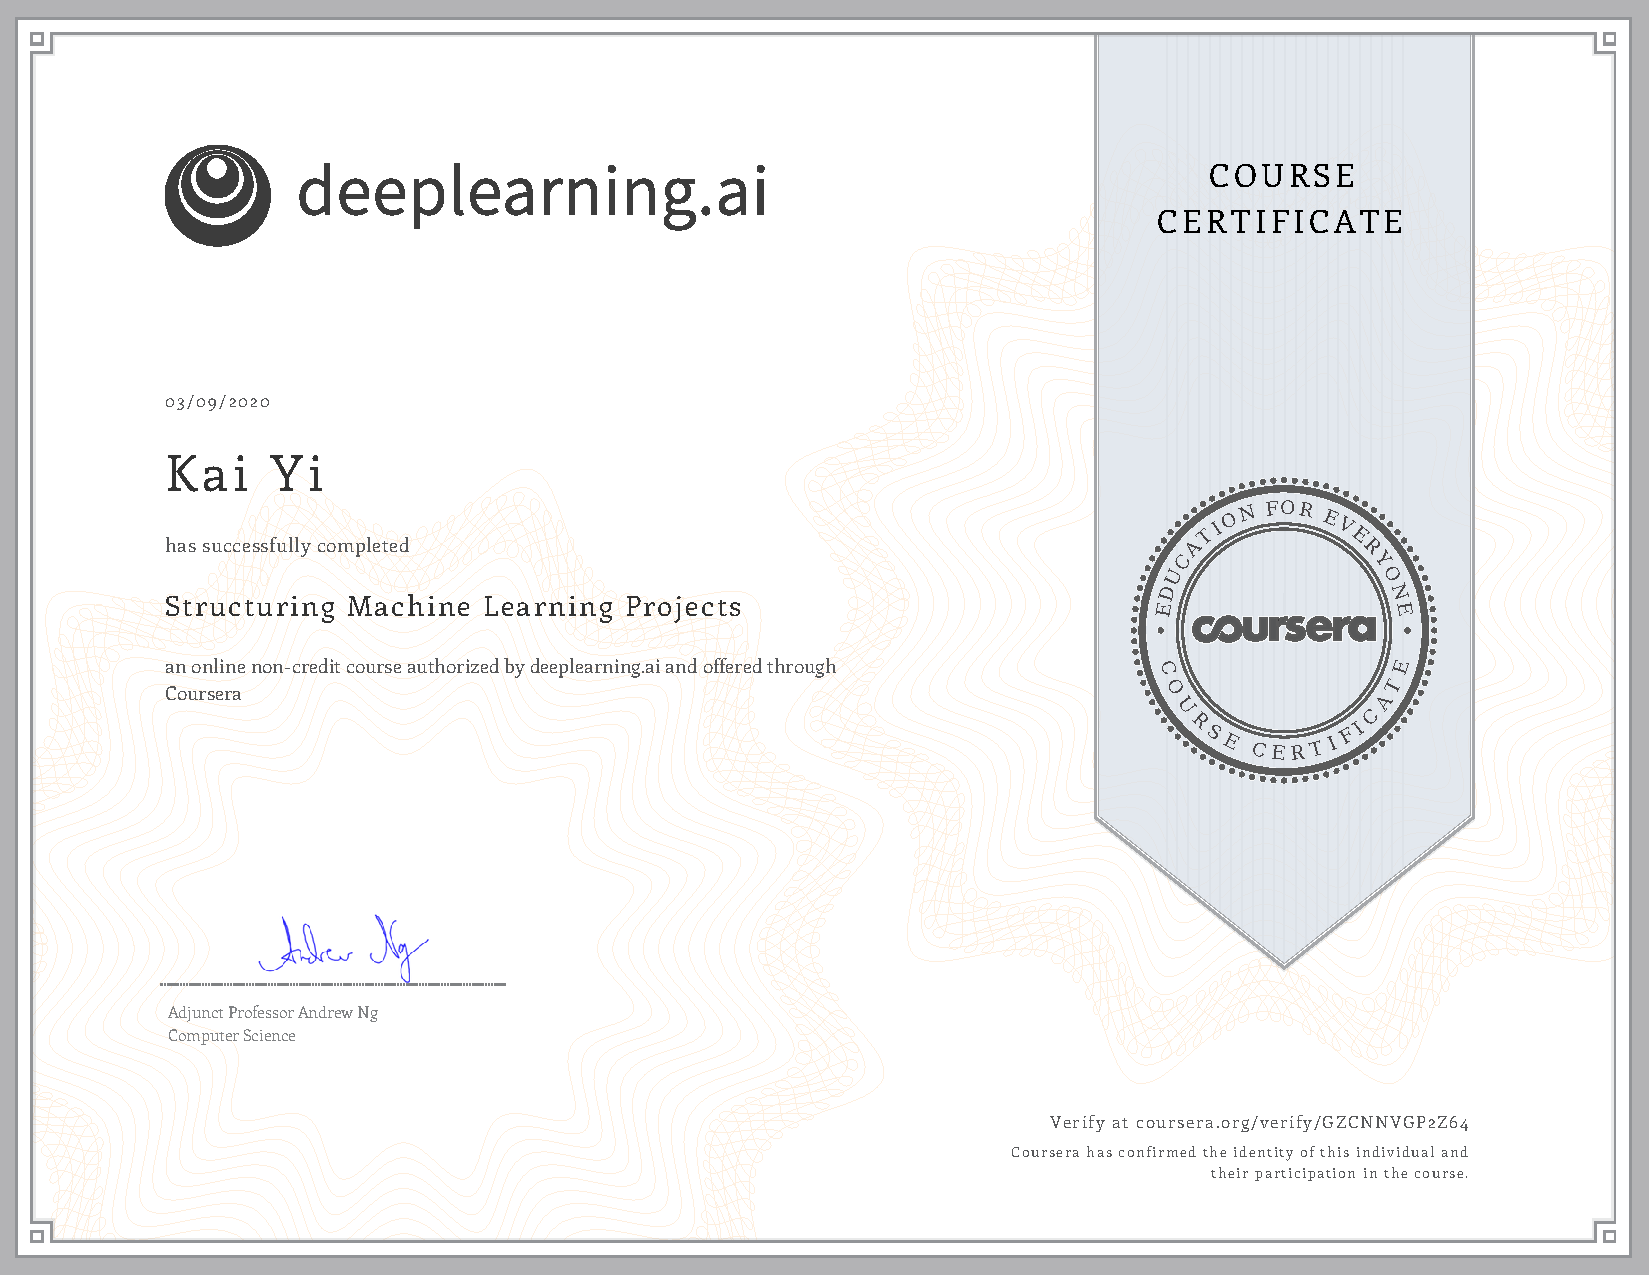
\includegraphics[width=1.0\textwidth]{img/C3-Certificate.pdf}
    \caption{Certificate of Structuring Machine Learning Projects. Obtained in Mar. 2020.}
    \label{C3-Certificate}
\end{figure}

\subsection{Course Overview}
According to the official site of this course, there are following key components:

\begin{itemize}
    \item Understand how to diagnose errors in a machine learning system.
    \item Be able to prioritize the most promising directions for reducing error.
    \item Understand complex ML settings, such as mismatched training sets, and comparing to and/or surpassing human-level performance.
    \item Know how to apply end-to-end learning, transfer learning, and multi-task learning.
\end{itemize}

\subsection{Machine Learning (ML) Strategy I}
\subsubsection{Why ML Strategy}
You have a lot of ideas for how to improve the accuracy of your deep learning system:

\begin{itemize}
    \item Collect more data.
    \item Collect more diverse training set.
    \item Train algorithm longer with gradient descent.
    \item Try different optimization algorithm (e.g. Adam)
    \item Try bigger network.
    \item Try smaller network.
    \item Try dropout.
    \item Add L2 regularization.
    \item Change network architecture (activation functions, nums of hidden units, etc)
\end{itemize}

This course will give you some strategies to help analyze your problem to go in a direction that will help you get better results.

\subsubsection{Orthogonalization}
Some deep learning developers know exactly what hyperparameter to tune in order to try to achieve one effect. This is a process we call orthogonalization.

In orthogonalization, you have some controls, but each control does a specific task and doesn't affect other controls.

For a supervised learning system to do well, you usually need to tune the knobs of your system to make sure that four things hold true -chain of assumptions in machine learning:

\begin{itemize}
    \item You'll have to fit training set well on cost function (near human level performance if possible). (If it's not achieved you could try bigger network, another optimization algorithm (like Adam)...)
    \item Fit dev set well on cost function. (If it's not achieved you could try regularization, bigger training set...)
    \item Fit test set well on cost function. (If it's not achieved you could try bigger dev set...)
    \item Performs well in real world. (If it's not achieved you could try to change dev set, change cost function...)
\end{itemize}

\subsubsection{Single Number Evaluation Metric}
It's better and faster to set a single number evaluation metric for your project before you start it.

Difference between precision and recall (in cat classification example):

\begin{itemize}
    \item Suppose we run the classifier on 10 images which are 5 cats and 5 non-cats. The classifier identifies that there are 4 cats, but it identified 1 wrong cat.
    \item Confusion matrix (Table \ref{confusion-matrix}).
\end{itemize}

\begin{table}[!htbp]
    \centering
    \begin{tabular}{c|c|c}
        \hline
        - & Predicted Cat & Predicted Non-Cat \\
        \hline
        Actual Cat & 3 & 2\\
        Actual Non-Cat & 1 & 4\\
        \hline
    \end{tabular}
    \caption{Confusion matrix.}
    \label{confusion-matrix}
\end{table}

\begin{itemize}
    \item Precision: percentage of true cats in the recognized result: P = 3/(3+1)
    \item Recall: percentage of true recognition cat of the all cat predictions: R = 3/(3+2)
    \item Accuracy: (3+4)/10
\end{itemize}

Using a precision/recall for evaluation is good in a lot of cases, but separately they don't tell you which algorithm is better. E.g. (Table \ref{pr-classifiers}):

\begin{table}[!htbp]
    \centering
    \begin{tabular}{c|c|c}
        \hline
        Classifier & Precision & Recall \\
        \hline
        A & 95\% & 90\%\\
        B & 98\% & 85\%\\
        \hline
    \end{tabular}
    \caption{Precision and recall of two classifiers.}
    \label{pr-classifiers}
\end{table}

A better thing is to combine precision and recall in one single (real) number evaluation metric. There is a metric called F1 score, which combines them:

\begin{itemize}
    \item You can think of F1 score as an average of precision and recall (Equation \ref{f1-matrix}).
\end{itemize}

\begin{equation}\label{f1-matrix}
    F1 = \frac{2}{\frac{1}{P} + \frac{1}{R}}
\end{equation}

\subsubsection{Satisfying and Optimizing Metric}
Its hard sometimes to get a single number evaluation metric. E.g. (Table \ref{pr-mixclassify}):

\begin{table}[!htbp]
    \centering
    \begin{tabular}{c|c|c}
        \hline
        Classifier & F1 & Running Time \\
        \hline
        A & 90\% & 80 ms\\
        B & 92\% & 95 ms\\
        C & 92\% & 1,500 ms\\
        \hline
    \end{tabular}
    \caption{F1 and Running Time of 3 classifiers.}
    \label{pr-mixclassify}
\end{table}

So we can solve that by choosing a single optimizing metric and decide that other metrics are satisfying. E.g.:

\begin{itemize}
    \item Maximize 1 (F1 here) \ \ \# optimizing metric (one optimizing metric)
    \item subject to N-1 satisfying metrics (running time < 1, 000 here)\ \ \# (N-1 satisfying metrics)
\end{itemize}

\subsubsection{Train/dev/test Distributions}
Dev and test sets have to come from the same distribution.

Choose dev set and test set to reflect data that you expect to get in the future and consider important to do well on.

Setting up the dev set, as well as the validation metric is really defining what target you want to aim at.

\subsubsection{Size of the Dev and Test Sets}
An old way of splitting the data was 70\% training, 30\% test or 60\% training, 20\% dev and 20\% test.

The old way was valid for a number of examples ~<100000.

In the modern deep learning if you have a million or more examples a reasonable split wound be 98\% training, 1\% dev and 1\% test.

\subsubsection{When to Change Dev/Test Sets and Metrics}
Let's take an example. In a cat classification example we have these matric results (Table \ref{when2change}):

\begin{table}[!htbp]
    \centering
    \begin{tabular}{c|c}
        \hline
        Algorithm &  Classification Error\\
        \hline
        A & 3\% error (but a lot of porn images are treated as cat images here)\\
        B & 5\% error\\
        \hline
    \end{tabular}
    \caption{Example of "When to Change Dev/Test Sets and Metrics".}
    \label{when2change}
\end{table}

In the above example if we choose the best algorithm by metric it would be "A", but if the users decide if will be "B".

Thus in this case, we want and need to change our metric. The solution is to add weights to select from different criterion.

Conclusion: If doing well on your metric + dev/test set doesn't correspond to doing well in your application, change your metric and/or dev/test set.

\subsubsection{Why human-level performance?}
We compare to human-level performance because of two main reasons:
\begin{itemize}
    \item Because of advances in deep learning, machine learning algorithms are suddenly working much better and so it has become much more feasible in a lot of application areas for machine learning algorithms to actually become competitive with human-level performance.
    \item It turns out that the workflow of designing and building a machine learning system is much mor efficient when you're trying to don something that humans can also do.
\end{itemize}

After an algorithm reaches the human level performance the progress of accuracy slow don \ref{humanlevelperformance}.

\begin{figure}
    \centering
    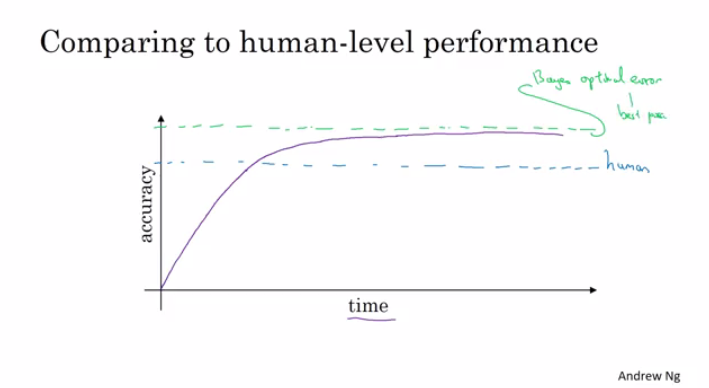
\includegraphics[width=1.0\textwidth, trim={20 50 0 50}, clip]{img/c2/human-level_performance.png}
    \caption{Comparing to human level performance.}
    \label{humanlevelperformance}
\end{figure}

You won't surpass an error that's called "Bayes optimal error".

There isn't much error range between human-level error and Bayes optimal error in computer vision tasks.

Humans are quite good at a lot of tasks. So as long as the machine learning method is worse than humans, you can:

\begin{itemize}
    \item Get labeled data from humans.
    \item Gain insight from manual error analysis: why did a person get it right?
    \item Better analysis of bias/variance.
\end{itemize}

\subsubsection{Avoidable Bias}
Suppose that the cat classification algorithm gives these results (Table \ref{avoidable-bias}):

\begin{table}[!htbp]
    \centering
    \begin{tabular}{c|c|c}
        \hline
        Humans & 1\% & 7.5\% \\
        Training Error & 8\% & 8\%\\ 
        Dev Error & 10\% & 10\%\\
        \hline
    \end{tabular}
    \caption{Example of avoidable bias.}
    \label{avoidable-bias}
\end{table}

In the left example, because the human level error is 1\% then we have to focus on the bias.

In the right example, because the human level error is 7.5\% then we have to focus on the variance.

The human-level error as a proxy (estimate) for Bayes optimal error. Bayes optimal error is always less (better), but human-level in most cases is not far from it.

Avoidable bias = Training error - Human (Bayes) error

Variance = Dev error - Training error

\subsubsection{Understanding Human-Level Performance}
When choosing human-level performance, it has to be chosen in the terms of what you want to achieve with the system.

You might have multiple human-level performances based on the human experience. Then you choose the human-level performance (proxy for Bayes error) that is more suitable for the system you're trying to build.

Improving deep learning algorithms is harder once you reach a human-level performance.

Summary of bias/variance with human-level performance:

\begin{itemize}
    \item Human-level error (proxy for Bayes error). Calculate avoidable bias = training error - human-level error. If avoidable bias difference is the bigger, then it's bias problem and you should use a strategy for bias resolving.
    \item Training error. Calculate variance = dev error - training error. If variance difference is bigger, then you should use a strategy for variance resolving.
    \item Dev error.
\end{itemize}

So having an estimate of human-level performance gives you an estimate of Bayes error. And this allows you to more quickly make decisions as to whether you should focus on trying to reduce a bias or trying to reduce the variance of your algorithm.

These techniques will tend to work well until you surpass human-level performance, whereupon you might no longer have a good estimate of Bayes error that still helps you make this decision really clearly.

\subsubsection{Surpassing Human-Level Performance}
In some problems, deep learning has surpassed human-level performance. Like:

\begin{itemize}
    \item Online advertising
    \item Product recommendation
    \item Load approval
\end{itemize}

The listed examples are not natural perception task. Humans are far better in natural perception tasks like computer vision and speech recognition. It's harder for machines to surpass human-level performance in natural perception task. But there are already some systems that achieved it.

\subsubsection{Improving Your Model Performance}
To improve your deep learning supervised system follow these guidelines:

\begin{itemize}
    \item[i.] Look at the difference between human level error and the training error - avoidable bias.
    \item[ii.] Look at the difference between the dev/test set and training set error - variance.
    \item[iii.] If avoidable bias is large you have these options: 1) Train bigger model; 2) Train longer/better optimization algorithm (like Momentum, RMSprop, Adam); 3) Find better NN architecture/hyperparameters search.
    \item[iv.] If variance is large you have these options: 1) Get more training data; 2) Regularization (L2, dropout, data augmentation); 3) Find better NN architecture/hyperparameters search.
\end{itemize}

\subsection{Machine Learning Strategy II}
\subsubsection{Carrying Out Error Analysis}
Error analysis - process of manually examining mistakes that your algorithm is making. It can give you insights into what to do next. E.g.:

\begin{itemize}
    \item In the cat classification example, if you have 10\% error on your dev set and you want to decrease the error.
    \item You discovered that some of the mislabeled data are dog pictures that look like cats. Should you try to make your cat classifier do better on dogs (this could take some weeks)?
    \item Error analysis approach:
    \begin{itemize}
        \item Get 100 mislabeled dev set examples at random.
        \item Count up how many are dogs.
        \item If 5 of 100 are dogs then training your classifier to do better on dogs will decrease your error up to 9.5\% (called ceiling), which can be too little.
        \item If 50 of 100 are dogs then you could decrease your error up to 5\%, which is reasonable and you should work on that.
    \end{itemize}
\end{itemize}

Based on the above example, error analysis helps you to analyze the error before taking an action that could take a lot of time with no need.

Sometimes, you can evaluate multiple error analysis ideas in parallel and choose the best idea. Create a spreadsheet to do that and decide, e.g. (Table \ref{error-analysis}):

\begin{table}[!htbp]
    \centering
    \begin{tabular}{c|c|c|c|c|c}
        \hline
        Image & Dog & Great Cats & Blurry & Instagram Filters & Comments \\
        \hline
        1 & $\surd$ & & & $\surd$ & Pitbull\\
        2 & $\surd$ & & $\surd$ & $\surd$ &\\
        3 &&&&& Rainy day at zoo\\
        4 && $\surd$&&&\\
        $\cdots$ &&&&&\\
        \hline
        \% totals & 8\% & 43\% & 61\% & 12\% & \\
        \hline
    \end{tabular}
    \caption{Spreadsheet of 100 selected images for error analysis.}
    \label{error-analysis}
\end{table}

In the above example you will decide to work on great cats or blurry images to improve your performance.

This quick counting procedure, which you can often do in, at most, small numbers of hours can really help you make much better prioritization decisions, and understand how promising different approaches are to work on.

\subsubsection{Cleaning Up Incorrectly Labeled Data}
Deep learning algorithms are quite robust to random errors in the training set but less robust to systematic errors. But it's OK to go and fix these labels if you can.

If you want to check for mislabeled data in dev/test set, you should also try error analysis with the mislabeled column. E.g. (Table \ref{mislabeled}):

\begin{table}[!htbp]
    \centering
    \begin{tabular}{c|c|c|c|c|c}
        \hline
        Image & Dog & Great Cats & Blurry & Mislabeled & Comments \\
        \hline
        1 & $\surd$ & & & $\surd$ & Pitbull\\
        2 & $\surd$ & & $\surd$ & $\surd$ &\\
        3 &&&&& Rainy day at zoo\\
        4 && $\surd$&&&\\
        $\cdots$ &&&&&\\
        \hline
        \% totals & 8\% & 43\% & 61\% & 12\% & \\
        \hline
    \end{tabular}
    \caption{Spreadsheet of 100 selected images for error analysis.}
    \label{mislabeled}
\end{table}

Then: If overall dev set error is 10\%, then errors due to incorrect data is 0.6\% while the errors due to other causes is 9.0\%. Thus you should focus on the 9.4\% error rather than the incorrect data.

Consider these guidelines while correcting the dev/test mislabeled examples:

\begin{itemize}
    \item Apply the same process to your dev and test sets to make sure they continue to come from the same distribution.
    \item Consider examining examples your algorithm got right as well as ones it got wrong. (Not always done if you reached a good accuracy)
    \item Train and (dev/test) data may now come from a slightly different distributions.
    \item It's very important to have dev and test sets to come from the same distribution. But it could be OK for a train set to come from slightly different distribution.
\end{itemize}

\subsubsection{Build You First System Quickly, Then Iterate}
The steps you take to make your deep learning project:

\begin{itemize}
    \item Setup dev/test set and metric.
    \item Build initial system quickly.
    \item Use bias/variance analysis \& error analysis to prioritize next steps.
\end{itemize}

\subsubsection{Training and Testing on Different Distributions}
A lot of teams are working with deep learning applications that have training sets that are different from the dev/test sets due to the hunger of deep learning to data.

There are some strategies to follow up when training set distribution differs from dev/test sets distribution:

\begin{itemize}
    \item Option I (not recommended): shuffle all the data together and extract randomly training and dev/test sets.
    \begin{itemize}
        \item Advantages: all the sets now come from the same distribution.
        \item Disadvantages: the other (real world) distribution that was in the dev/test sets will occur less in the new dev/test sets and that might be not what you want to achieve.
    \end{itemize}
    \item Option II: take some of the dev/test set examples and add them to the training set.
    \begin{itemize}
        \item Advantages: the distribution you care about is the target now.
        \item Disadvantages: the distributions in training and dev/test sets are now different. But you will get a better performance over a long time.
    \end{itemize}
\end{itemize}

\subsubsection{Bias and Variance With Mismatched Data Distributions}
Bias and variance analysis changes when training and dev/test set is from the different distribution.

Example: the cat classification example. Suppose you've worked in the example and reached this:

\begin{itemize}
    \item Human error: 0\%
    \item Train error: 1\%
    \item Dev error: 10\%
\end{itemize}

In this example, you may think this is a variance problem, but because the distributions aren't the same you can't tell for sure. Because it could be that train set was easy to train on, but the dev set was more difficult.

To solve this issue, we create a new set called train-dev set as a random subset of the training set (so it has the same distribution) and we get:

\begin{itemize}
    \item Human error: 0\%
    \item Train error: 1\%
    \item Train-dev error: 9\%
    \item Dev error: 10\%
\end{itemize}

Now we are sure that this is a high variance problem.

Suppose we have a different situation:

\begin{itemize}
    \item Human error: 0\%
    \item Train error: 1\%
    \item Train-dev error: 1.5\%
    \item Dev error: 10\%
\end{itemize}

In this case, we have something called \textit{data mismatch} problem.

Conclusions:

\begin{itemize}
    \item Human-level error (proxy for Bayes error)
    \item Train error
    \begin{itemize}
        \item Calculate \textit{avoidable bias = training error - human level error}.
        \item If the difference is big then its Avoidable bias problem then you should use a strategy for high bias.
    \end{itemize}
    \item Train-dev error
    \begin{itemize}
        \item Calculate \textit{variance = training-dev error - training error}.
        \item If the difference is big then its high variance problem then you should use a strategy for solving it.
    \end{itemize}
    \item Dev error
    \begin{itemize}
        \item Calculate \textit{data mismatch = dev error - train-dev error}.
        \item If difference is much bigger then train-dev error its Data mismatch problem.
    \end{itemize}
    \item Test error
    \begin{itemize}
        \item Calculate \textit{degree of overfitting to dev set = test error - dev error}.
        \item Is the difference is big (positive) then maybe you need to find a bigger dev set (dev set and test set come from the same distribution, so the only way for there to be a huge gap here, for it to do much better on the dev set than the test set, is if you somehow managed to overfit the dev set).
    \end{itemize}
\end{itemize}

Unfortunately, there aren't many systematic ways to deal with data mismatch. There are some things to try about this in the next section.

\subsubsection{Addressing Data Mismatch}
There aren't completely systematic solutions to this, but there are some things you could try.

\begin{itemize}
    \item Carry out manual error analysis to try to understand the difference between training and dev/test sets.
    \item Make training data more similar, or collect more data similar to dev/test sets.
\end{itemize}

If your goal is to make the training data more similar to your dev set one of the techniques you can use is \textit{artificial data synthesis} that can help you make more training data.

\begin{itemize}
    \item Combine some of your training data with something that can convert it to the dev/test set distribution. E.g.:
    \begin{itemize}
        \item Combine normal audio with car noise to get audio with car noise example.
        \item Generate cars using 3D graphics in a car classification example.
    \end{itemize}
    \item Be cautious and bear in mind whether or not you might be accidentally simulating data only from a tiny subset of the space of all possible examples because your NN might overfit these generated data (like particular car noise or a particular design of 3D graphics cars).
\end{itemize}

\subsubsection{Transfer Learning}
Apply the knowledge you took in a task A and apply it in another task B.

For example, you have trained a cat classifier with a lot of data, you can use the part of the trained NN to solve medical image classification problem.

To do transfer learning, delete the last few layers of NN and theis weights and:

\begin{itemize}
    \item Option I: If you have a small data set - keep all the other weights as a fixed weights. Add a new last layer(-s) and initialize the new layer weights and feed the new data to the NN and learn the new weights.
    \item Option II: If you have enough data you can retrain all the weights.
\end{itemize}

Option I and II are called \textbf{fine-tuning} and training on task A called \textbf{pretraining}.

When transfer learning make sense:

\begin{itemize}
    \item Task A and B have the same input X (e.g. image, audio).
    \item You have a lot of data for the task A you are transferring from and relatively less data for the task B your transferring to.
    \item Low level features from task A could be helpful for learning task B.
\end{itemize}

\subsubsection{Multi-Task Learning}
Whereas in transfer learning, you have a sequential process where you learn from task A and then transfer that to task B. In multi-task learning, you start off simultaneously, trying to have one neural network do several things at the same time. And then each of these tasks helps hopefully all of the other tasks.

Example: You want to build an object recognition system that detects pedestrians, cars, stop signs and traffic lights (image has multiple labels).

Then Y shape will be (4,m) because we have 4 classes and each one is a binary one.

Then.

\begin{equation}
\begin{aligned}
    Cost &= \frac{1}{m} \sum^m_{i=1}\sum_{j=1}^{4} L(\hat{y}^{i}_j, y^{i}_j), \ \ i = 1\to m, j = 1\to 4\\
    L &= - y^i_j * \log (\hat{y}^i_j) - (1 - y^i_j) * \log (1 - \hat{y}^i_j)\\
\end{aligned}
\end{equation}

In the above example, you could have trained 4 neural networks separately but if some of the earlier features in NN can be shared among these different types of objects, then you find that training one NN to do four things results in better performance than training 4 completely separate NNs to do the four tasks separately.

Multi-task learning will also work if y isn't complete for some labels. E.g.:

\begin{lstlisting}
Y = [1 ? 1 ...]
    [0 0 1 ...]
    [? 1 ? ...]
\end{lstlisting}

In the above case, it will do good with the missing data, just the loss function will be different:

\begin{equation}
    \begin{aligned}
        L &= - y^i_j * \log (\hat{y}^i_j) - (1 - y^i_j) * \log (1 - \hat{y}^i_j)\ \  for\  all \ j \ which \  y^i_j != ?\\
    \end{aligned}
\end{equation}

Multi-task learning makes sense:

\begin{itemize}
    \item Training on a set of tasks that could benefit from having shared lower-level features.
    \item Usually, amount of data you have for each task is quite similar.
    \item Can train a big enough network to do well on all the tasks.
\end{itemize}

If you can train a big enough NN, the performance of the multi-task learning compared to splitting the tasks is better.

Today transfer learning is used more often than multi-task learning. But in the area of computer vision, multi-task learning is widely adapted.

\subsubsection{What Is End-to-end Deep Learning}
Some systems have multiple stages to implement. An end-to-end deep learning system implements all these stages with a single NN. E.g.:

\begin{itemize}
    \item Speech recognition system:
\begin{lstlisting}[language=python]
# non-end-to-end system
Audio ---> Features --> Phonemes --> Words --> Transcript    
# end-to-end deep learning system
Audio ---------------------------------------> Transcript    
\end{lstlisting}
    \item End-to-end deep learning gives data more freedom, it might not use phonemes when traning.
\end{itemize}

To build the end-to-end deep learning system that works well, we need a big dataset (more data then in non end-to-end system). If we have a small dataset the ordinary implementation could work just fine.

Another example of end-to-end learning:

\begin{itemize}
    \item Face recognition system:
\begin{lstlisting}[language=python]
# end-to-end deep learning system
Image ---------------------> Face recognition
# deep learning system - best approach for now
Image --> Face detection --> Face recognition    
\end{lstlisting}
    \item In practice, the best approach is the second one for now.
    \item In the second implementation, it's a two steps approach where both parts are implemented using deep learning.
    \item Its working well because it's harder to get a lot of pictures with people in front of the camera than getting faces of people and compare them.
    \item In the second implementation at the last step, the NN takes two faces as an input and outputs if the two faces are the same person or not (Siamese Neural Network\cite{koch2015siamese}).
\end{itemize}

Example 3:

\begin{itemize}
    \item Machine translation system:
\begin{lstlisting}[language=python]
# non-end-to-end system
English --> Text analysis --> ... --> French    
# end-to-end deep learning system - best approach
English ----------------------------> French    
\end{lstlisting}
    \item Here end-to-end deep leaning system works better because we have enough data to build it.
\end{itemize}

Example 4:

\begin{itemize}
    \item Estimating child's age from the x-ray picture of a hand:
\begin{lstlisting}[language=python]
# non-end-to-end system - best approach for now
Image --> Bones --> Age   
# end-to-end deep learning system
Image ------------> Age    
\end{lstlisting}
    \item In this example non-end-to-end system works better because we don't have enough data to train end-to-end system.
\end{itemize}

\subsubsection{Whether to Use End-to-end Deep Learning}
Pros of end-to-end deep learning:
\begin{itemize}
    \item Let the data speak. By having a pure machine learning approach, your NN learning input from X to Y may be more able to capture whatever statistics are in the data, rather than being forced to reflect human preconceptions.
    \item Less hand-designing of components needed.
\end{itemize}

Cons of end-to-end deep learning:
\begin{itemize}
    \item May need a large amount of data.
    \item Excludes potentially useful hand-design components (it helps more on the smaller dataset).
\end{itemize}

Applying end-to-end deep learning:
\begin{itemize}
    \item Key question: Do you have sufficient data to learn a function of the \textbf{complexity} needed to map x to y?
    \item When applying supervised learning you should carefully choose what types of X to Y mappings you want to learn depending on what task you can get data for.
\end{itemize}
\newpage